\documentclass[12pt, a4paper, one side]{article}
\usepackage[utf8]{inputenc}
\usepackage[french]{babel}
\usepackage{biblatex}
\usepackage{listings}
\usepackage{xcolor}
\usepackage{hyperref}
\usepackage{graphicx}

\bibliography{reference}

\usepackage{comment}

\lstset{
    basicstyle=\itshape,
    xleftmargin=3em,
    literate={->}{$\rightarrow$}{2}
        {^}{$\uparrow$}{1}
        {↓}{$\downarrow$}{1},
    morekeywords={method_body},
    basicstyle=\small
}

\definecolor{codegreen}{rgb}{0,0.6,0}
\definecolor{codegray}{rgb}{0.5,0.5,0.5}
\definecolor{codepurple}{rgb}{0.58,0,0.82}
\definecolor{backcolour}{rgb}{0.95,0.95,0.92}

\lstdefinestyle{mystyle}{
    commentstyle=\color{codegreen},
    keywordstyle=\color{magenta},
    numberstyle=\tiny\color{codegray},
    breakatwhitespace=false,
    breaklines=true,
    captionpos=b,
    keepspaces=true,
    numbers=left,
    numbersep=5pt,
    showspaces=false,
    showstringspaces=false,
    showtabs=false,
    tabsize=2,
    extendedchars=true
}

\newcommand{\paragraphln}[1]{\paragraph{#1}\mbox{}\\}



\title{Documentation de l'extension}
\author{}
\date{}

\begin{document}

    \maketitle

    \begin{center}
        Valentin Laclautre, Anthony Dard, Damien Trouche, Martin Gangand, Basel Darwish Jzaerly
    \end{center}

    \tableofcontents

    \section{Spécifications}
    \subsection{Compilation de programmes Deca en executable pour la JVM}
    \subsubsection{Commande decac}
    \textbf{decac [[-p $\mid$ -v $\mid$ -java] [-n] [-r X] [-d]* [-P] [-w] $<$fichier deca$>$...] $\mid$ [-b]}
    \\

    L'option -java spécifie au compilateur qu'on souhaite compiler un programme Deca en executable pour la machine virtuelle Java.
    Ainsi, on obtient avec cette obtion un fichier .class executable par la JVM au lieu d'un fichier .ass (executable IMA). Les conventions de nommage sont les mêmes, c'est-à-dire que le nom du fichier compilé est celui du programme Deca, seule l'extension du fichier change.

    Cependant il y a quelques réstrictions. En effet, l'utilisation de code Java dans une méhode Deca impose une compilation vers la JVM (une erreur est renvoyée sinon). De plus la compilation vers la JVM impose qu'il n'y ai pas de méthode en Assembleur. (cf Limitations pour plus de précisions)

    \subsubsection{Spécification de compilation}
    La compilation se fait de la même manière que pour la machine IMA au detail près qu'au lieu d'appeler nos méthodes de compilation pour la machine abstraite IMA, le compilateur utilise la bibliothèque ASM\cite{ASM} pour la génération du bytecode.

    \subsection{Appel de code Java en Deca}
    Cette section précise les spécifications liées à l'appel de code Java en Deca.
    \subsubsection{Grammaire Deca pour l'appel de code Java}
    Une règle est ajoutée à la passe 3 pour prendre en compte les méthodes "Java"
    \begin{lstlisting}
method_body↓env_type↓env_exp↓env_exp_params↓class↓return
            -> MethodJavaBody [ StringLiteral ]
    \end{lstlisting}

    \subsubsection{Utilisation}
    L'utilisation de l'appel de code Java en Deca est très similaire à l'appel de code assembleur. En effet, il suffit de déclarer une méthode de la même manière, c'est-à-dire une méthode dont le corps est une chaîne de caractères contenant du code Java et en utilisant le mot clé 'java' à la place de 'asm'.
    \\

    Il est possible d'envoyer une valeur qui se trouve dans le code deca vers le code java en utilisant les paramètres de la méthode deca. Un exemple d'utilisation se trouve dans src/test/deca/codegen/valid/custom/extension/*.
    \\

    Enfin, il est utile de rappeler qu'il est possible de compiler une classe écrite en deca et puis utiliser le bytecode généré dans un programme java. On note que le fichier deca source doit être dans le même répertoire que le fichier java afin que la compilation fonctionne. C'est une limitation de deca.

    \section{Analyse bibliographique}
    Dans cette section nous allons donner des détaills techniques sur la  \textbf{Java virtual machine JVM}.

    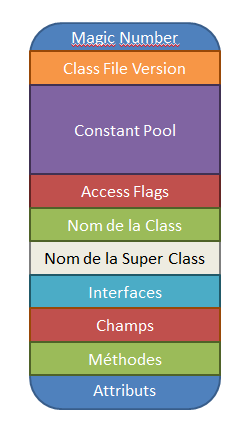
\includegraphics{JavaInternal}
    \\

    Let's cite! The Einstein's journal paper  \cite{ref_DexFormatvsJavabytecode}

    \section{Conception}
    \subsection{Documentation de conception}
    \subsubsection{Structure globale}
    \subsubsection{Choix d'implémentation}
    \subsection{Algorithmes utilisés}

    \section{Validation}
    \subsection{Protocole de validation}
    \subsection{Résultats}

    \section{Limitations}
    \subsection{Compatibilité Java-Deca}


    \printbibliography

\end{document}
